\section{Evaluation}
\label{sec:eval}

\lstMakeShortInline[mathescape=true]{|}

We have implemented analytic program repair in \toolname: a system for 
repairing type errors for a purely functional subset of \ocaml. Next,
we describe our implementation and an evaluation that addresses three 
questions:

\begin{itemize}
    \item \textbf{RQ1}: How \emph{accurate} are \toolname's predicted repairs? 
                        (\S~\ref{sec:eval:accuracy}) 
    \item \textbf{RQ2}: How \emph{efficiently} can \toolname synthesized fixes?
                        (\S~\ref{sec:eval:efficiency}) 
    \item \textbf{RQ3}: How \emph{useful} are \toolname's error messages? 
                        (\S~\ref{sec:eval:useful}) 
\end{itemize}

% \subsection{Implementation} \label{sec:eval:gen_method}

\mypara{Training Dataset}
%
For our evaluation, we use an \ocaml dataset gathered from an undergraduate
Programming Languages university course, previously used in related work
\citep{yunounderstand,Seidel:2017}. It consists of erroneous programs and their
subsequent fixes and is divided in two parts; the Spring 2014 class (\SPRING)
and the Fall 2015 class (\FALL). The homework required students to write 23
distinct programs that demonstrate a range of functional programming idioms, \eg
higher-order functions and (polymorphic) algebraic data types.

\mypara{Feature Extraction}
%
\toolname represents programs with BOAT vectors over 
a set of 416 features from each sub-expression in a 
program, including: 
%
45 local syntactic features.
%
315 contextual syntactic features. For each subexpression we
additionally extract the local syntactic features of its first 4
(left-to-right) children. In addition, we extract those features for its
ancestors, starting from its parent and going up to two more parent nodes.
    % If an expression does not have a ancestor or children, these features will
    % simply be disabled. If an expression has more than four children, the
    % classifiers will receive no information about the additional children.
    %
88 typing features. We support |int|s, |float|s, |char|s, |string|s, and
    the user-defined |expr|. These features are extracted for each
    sub-expression and its context.
% 
1 feature denoting the size of each subexpression.

\mypara{Dataset Cleaning}
%
We extract fixes as expressions replacements over a program pair using \diffsym.
A disadvantage of using \diffsym s with this dataset is that students may have
made many, potentially unrelated, changes between compilations; at some point
the ``fix'' becomes a ``rewrite''. These ``rewrites'' can potentially lead to
meaningless fix templates and error locations. We discard such outliers when the
fraction of subexpressions that have changed in a program is more than one
standard deviation above the mean, establishing a diff threshold of 40\%. We
also discard programs that have changes in 5 or more locations. Even
state-of-the-art multi-location repair techniques can't reproduce such ``fixes''
\citep{Saha_2019}. The discarded changes account for roughly 32\% of each
dataset, leaving 2,475 program pairs for \SPRING and 2,177 pairs for \FALL.
Throughout, we use \SPRING as a training set and \FALL as a test set.

\mypara{\dnn based Classifier}
%
\toolname's template prediction 
uses a multi-layer neural network \dnn based 
classifier that utilizes three fully-connected 
hidden layers of 512 neurons. The neurons use
rectified linear units (ReLU) as their activation 
function.
%
The \dnn was trained using \emph{early stopping} 
\cite{Hastie2009-bn}, where the training of a neural 
network is stopped when the accuracy on a distinct 
small part of the training set is not improved after 
a certain amount of epochs.
%
We used the \textsc{Adam} optimizer \citep{Kingma2014-ng}, 
a variant of stochastic gradient descent that has 
been found to converge faster, was used to train 
our \dnn; and we that amount to 5 \RJ{what amount?} 
and set the maximum number of epochs to 200. 

\subsection{Evaluation of Accuracy}

\label{sec:eval:accuracy}

Most developers will consider around five or six suggestions before
falling back to manual debugging \citep{Kochhar2016-oc}. 
%
Therefore, we consider \toolname's accuracy up to the \emph{top six} 
fix template prediction, \ie predicted fix templates that represent 
the user's actual fix. 

\mypara{Baselines}
%
We compare \toolname's \dnn based predictor against two baseline 
classifiers: a \random classifier that returns 
for each location it is presented, a template 
chosen uniformly at random from the 50 templates 
learned from the \SPRING training dataset and 
a \popular classifier that returns the most 
popular templates in the training set in 
decreasing order. 

\mypara{Results: Accuracy of Prediction}
%
\autoref{fig:accuracy-results} shows the accuracy results of our template
prediction experiments. The y-axis describes the fraction of \emph{erroneous}
sub-terms (locations) for which the actual repair was one of the top-K predicted 
repairs.
%
The naive baseline of selecting templates at random achieves 
\RandomTopOne\% Top-1 accuracy (\RandomTopSix\% Top-6), while 
the \popular classifier achieves a Top-1 accuracy of \PopularTopOne\%
(\PopularTopSix\% Top-6).
%
Our \dnn classifier significantly outperforms those naive 
classifiers, ranging from \DnnTopOne\% Top-1 accuracy to 
\DnnTopSix\% Top-6 accuracy. 
%
Interestingly, with only \dnn's first prediction, one
outperforms top 6 predictions of both \random and \popular.
%
The \random classifier's low performance is as expected.
%
The \popular classifier performs better: some homework assignments 
were shared between \SPRING and \FALL quarters and, while different 
groups of students solved these problems for each quarter, the novice
mistakes that they made seem to have a pattern. Thus, the most
\emph{popular ``fixes''} (and therefore the relevant templates) 
that were applied to \SPRING, are also popular in \FALL. 

% colors from http://colorbrewer2.org/?type=sequential&scheme=Blues&n=3
\definecolor{blue1}{HTML}{DEEBF7}
\definecolor{blue2}{HTML}{9ECAE1}
\definecolor{blue3}{HTML}{3182BD}
\definecolor{green1}{HTML}{E5F5E0}
\definecolor{green2}{HTML}{A1D99B}
\definecolor{green3}{HTML}{31A354}

\begin{figure}[t]
\centering
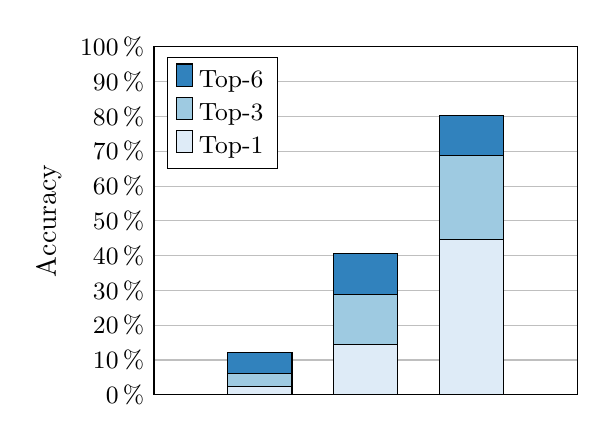
\begin{tikzpicture}
\begin{axis}[
  ybar stacked,
  % width=\linewidth,
  height=6cm,
  % title={Accuracy of Repair Template Prediction},
  ylabel={Accuracy},
  bar width=0.82cm,
  ymin=0.0,
  ymax=100.0,
  ytick={0.0, 10.0, 20.0, 30.0, 40.0, 50.0, 60.0, 70.0, 80.0, 90.0, 100.0},
  yticklabel={\pgfmathparse{\tick}\pgfmathprintnumber{\pgfmathresult}\,\%},
  ytick style={draw=none},
  ymajorgrids = true,
  symbolic x coords={random, popular, dnn},
  enlarge x limits=0.5,
  xtick=data,
  xtick style={draw=none},
  xticklabels={\random, \popular, \dnn},
  %x tick label style={rotate=45, anchor=north east},
  x tick label style={font=\small},
  y tick label style={font=\small},
  reverse legend,
  transpose legend,
  legend style={legend pos = north west, legend columns=4, font=\small},
]

\addplot[draw=black, fill=blue1] coordinates {(random, 2.35646958011996552) (popular, 14.438731790916881) (dnn, 44.64438731790917)};
\addlegendentry{Top-1}
\addplot[draw=black, fill=blue2] coordinates {(random, 3.6846615252784924) (popular, 14.395886889460153) (dnn, 24.250214224507282)};
\addlegendentry{Top-3}
\addplot[draw=black, fill=blue3] coordinates {(random, 6.212510711225363) (popular, 11.825192802056556) (dnn, 11.482433590402735)};
\addlegendentry{Top-6}

\end{axis}
\end{tikzpicture}
\caption{
  Results of our template prediction classifiers using the \emph{50 most
  popular} templates. We present the results up to the top 6 predictions, since
  our synthesis algorithm considers that many templates before falling to a
  different location.
}
\label{fig:accuracy-results}
\end{figure}


\begin{figure}[t]
  \centering
  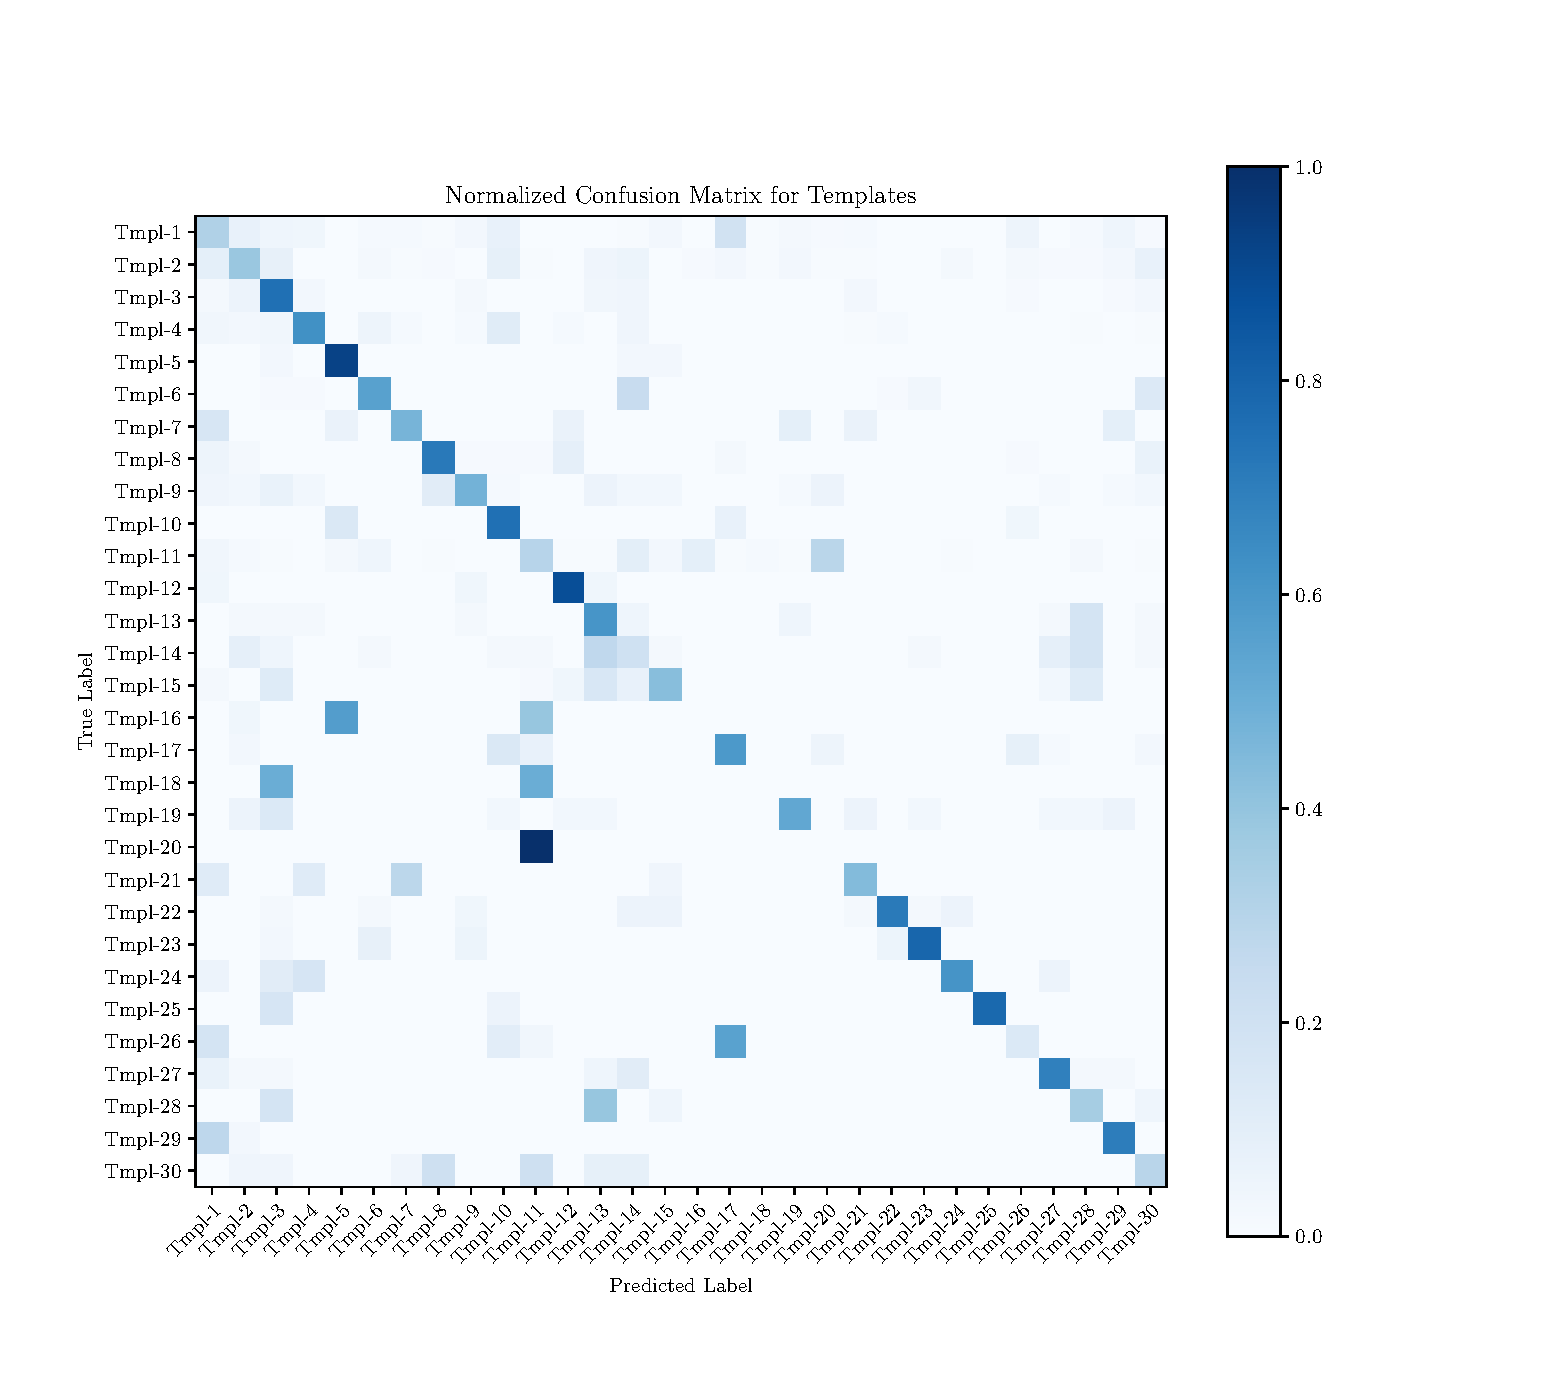
\includegraphics[trim={30 40 100 70},clip,width=\linewidth]{evaluation-conf-matrix.pdf}
  \caption{The confusion matrix of the \emph{top 30} templates. Bolder parts of
  the heatmap show templates that are often mis-predicted with another template.
  The bolder the diagonal is, the more accurate predictions we make.}
  \label{fig:conf-matrix}
\end{figure}

\mypara{Results: Template ``Confusion''}
%
We also compute the \emph{confusion matrix} of the each location's 
top prediction, to present what templates our models usually mix 
with each other and see if they generalize well between different 
groups of solutions. 
%
\autoref{fig:conf-matrix} shows the confusion matrix of the 
top 30 templates that were acquired from the training set 
and were tested on \FALL dataset.
%
We observe that most of the templates are predicted correctly 
and only a few of them are often mis-predicted for another template. 
%
For example, we see that programs that would require template 20 
to be fixed almost always are mis-predicted with template 11.

\GS{show those two templates, both ``let''s with some ``tuple'' in their ASTs}

\begin{framed}
  \noindent \toolname's learns correlations between program features and repair 
  templates, yielding almost \emph{2x higher} accuracy than the baseline;
  by abstracting programs into features, \toolname is able 
  to \emph{generalize} across years and different kinds of programs.
\end{framed}


\subsection{Evaluation of Efficiency}
\label{sec:eval:efficiency}
\label{subsec:eval:man_rep_qual_eval}

Next we evaluate the efficiency of \toolname by measuring how many 
programs it is able to generate a (well-typed) repair for.
%
Recall that the repair synthesis algorithm is guided by the 
repair template predictions.
%
To measure efficiency, we give the synthesizer \emph{60s} to 
compute a repair and timeout otherwise. (In general the procedure 
is undecidable, and we conjecture that a longer timeout will diminish 
the practical usability for novices.
%
In \autoref{tab:rite_naive}, we evaluate the efficiecy of \toolname
by comparing it against a baseline \naive implementation that, given 
the predicted fix location, attempts to synthesize a repair from the 
trivial ``hole'' template $\_$.

The first column of \autoref{tab:rite_naive} shows how many 
programs were completed on the time limit, while the second 
column how many returned a type-correct solution. 
%
We observe that using predicted templates for synthesis allows 
\toolname to generate type-correct repairs for almost 85\% of 
the programs, which is nearly 10 points hire than the \naive 
baseline. Also, for the programs that are completed within 
the time limit, \toolname needs an average of $8.81$ seconds 
to repair an erroneous program, while \naive takes 
\textbf{33\%} longer.

\begin{framed}
  \noindent \toolname can generate type-correct repairs 
  for the vast majority of ill-typed programs in under 
  \RJ{XXX}.
\end{framed}
  
% The 11.85\% of the programs that fail to be repaired within that amount of time
% fall in the case of the combined failure of our predictive models to give high
% confidence scores to the correct locations and templates, thus making synthesis
% very expensive.

\begin{table}
  \centering
  \begin{tabular}{l|ccc}
    Classifier & Completed & Repair Rate & Time (sec) \\
    \hline
    \naive   & 77.86\% & 74.78\% & 11.72 \\
    \toolname & 88.15\% & 84.80\% & 8.81 \\
  \end{tabular}
  \caption{Experimental results of \toolname's synthesis.}
  \label{tab:rite_naive}
\end{table}

\GS{here the \seminal - \toolname - \naive comparison}

%%%%%%%%%%%%%%%%%%%%%%%%%%%%%%%%%%%%%%%%%%%%%%%%%%%%%%%%%%%%%%%%%%%%%%%%%%%%%%%
%%%%%%%%%%%%%%%%%%%%%%%%%%%%%%%%%%%%%%%%%%%%%%%%%%%%%%%%%%%%%%%%%%%%%%%%%%%%%%%
%%%%%%%%%%%%%%%%%%%%%%%%%%%%%%%%%%%%%%%%%%%%%%%%%%%%%%%%%%%%%%%%%%%%%%%%%%%%%%%
%%%%%%%%%%%%%%%%%%%%%%%%%%%%%%%%%%%%%%%%%%%%%%%%%%%%%%%%%%%%%%%%%%%%%%%%%%%%%%%

\subsection{Evaluation of Usefulness}
\label{sec:eval:useful}

Finally, the ultimate proof of the pudding is in whether the repair-based 
error messages generated by \toolname were actually useful to novices.
%
To assess the quality of \toolname's repairs, we conducted an online human
study with 29 participants. 
%
Each participant was asked to evaluate the quality of the program fixes 
and their locations against a state-of-the-art baseline 
(\seminal ~\citep{Lerner2007-dt}). 
%
For each program, beyond the two repairs, participants were presented
with the original ill-typed program, along with the standard \ocaml 
compiler's error message and a short description of what the original 
author of the program intended it to do. 
%
From this study, we found that both the edit locations and final 
repairs produced by \toolname were better than those produced by 
\seminal~\citep{Lerner2006-pj, Lerner2007-dt}, a state-of-the-art
\ocaml repair tool, in a statistically significant manner.

\mypara{User Study Setup}
%
Study participants were recruited from \emph{two public research
institutes removed for blind review}. The study was also advertised on Twitter.
To be included for analysis, participants had to assess the quality of, and give
comprehensible bug descriptions for, at least 5 / 10 stimuli. The study took around
25 minutes to complete. For compensation, participants had the option to enter a
drawing for an Amazon Echo voice assistant. In total, there were
29 valid participants.

To create the stimuli, a corpus of 21 buggy programs were randomly selected from
1834 type-correct synthesized programs in our dataset. From this corpus, each
participant was then shown 10 randomly-selected programs. Along with each buggy
program, participants were also shown two candidate repairs: one generated by
\toolname and one by \seminal. For both algorithms, we used the highest-ranked
solution returned. Participant were always unaware which tool generated which
candidate patch. Participants were then asked to assess the quality of each
candidate repair on a Likert scale of 1 to 5. They were further asked for a
binary assessment of the quality of each repair's edit location.
We also collected self-reported estimates of both programming and
\ocaml-specific experience as well as qualitative data assessing factors
influencing each participant's subjective judgment of repair quality.
From the 29 participants, we collected 554 patch quality assessments, 277 each
for \toolname and \seminal generated repairs.

%\begin{figure}
%  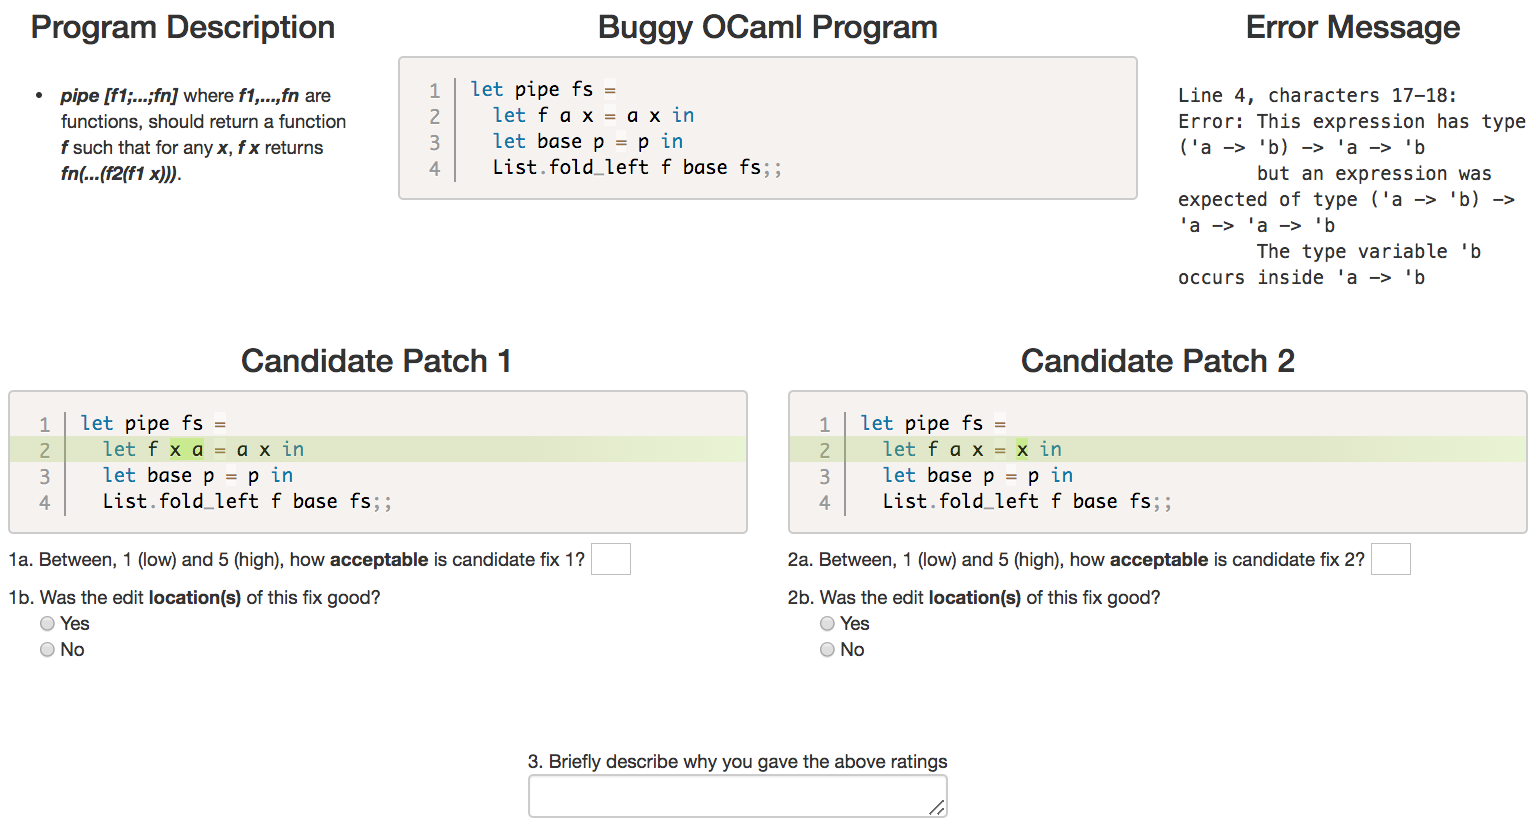
\includegraphics[width=8cm]{SampleStimuli.png}
%  \caption{A sample stimulus used for assessing repair quality.}
%  \label{fig:stimulus}
%\end{figure}

\mypara{Results}
%
In a statistically significant manner, humans perceive that
\toolname's fault localization and final repairs are both 
of higher quality than those produced by \seminal ($p=0.030$ 
and $p=0.024$ respectively)~\footnote{All tests for statistical 
significance used the Wilcoxon signed-rank test.}.
%
Regarding fault localization, we find that humans agreed
with \toolname-identified edit locations 81.6\% of the time 
but only agreed with those of \seminal only 74.0\% of the time. 
%
% This 10\% increase is important because \ME{You should explain why this matters.}
%
As for the final repair, humans also prefer \toolname's patches
to those produced by \seminal. Specifically, \toolname's repairs 
achieved an average quality rating of 2.41/5 while \seminal's 
repairs had an average rating of only 2.11/5, a 14\% increase ($p=0.030$),
showing a statistically significant improvement over \seminal.
%
This improvement shown by our data-driven method is especially 
significant because \seminal incorporates several expert-guided 
heuristics for improving the quality of error messages by biasing 
its reports towards simpler and more useful ones. 
%
Thus, our results demonstrate that data can be an unreasonably 
effective tool in the quest for better error messages.

% Indicate that 15\% better is still very
% useful for students, perhaps by citing something.

\begin{figure*}
\begin{subfigure}[t]{.38\textwidth}
\begin{center}
\textbf{Programming Task:}
\end{center}
\texttt{wwhile(f, b)} should return $x$ where
there exist values $v_0,...,v_n$ such that:
$b = v_0$, $x = v_n$, and
for each $i$ between 0 and $n-2$, we have $f v_i = (v_i+1, true)$
and $f v_n-1 = (v_n, false)$.
\begin{center}
\textbf{Buggy Student Solution:}
\end{center}
\begin{compactcode}
let rec wwhile (f, b) =
let (b', c') = f b in if c' = true
then wwhile __(f b')__ else b';;
\end{compactcode}
\begin{center}
\textbf{\toolname Repair:}
\end{center}
\begin{compactcode}
           ...__(f, b')__...
\end{compactcode}
\begin{center}
\textbf{\seminal Repair:}
\end{center}
\begin{compactcode}
     ...__((f b'); [[...]]))__...
\end{compactcode}
\caption{Humans perceived \toolname's repair to be
better than \seminal ($p=0.002$): With 12 responses, \toolname's
repair had a mean score of 4.5/5 compared to \seminal's
score of 1.1/5.}
\label{subfig:good1}
\end{subfigure}\hfill
\begin{subfigure}[t]{.1\textwidth}
\end{subfigure}\hfill
\begin{subfigure}[t]{.28\textwidth}
\begin{center}
\textbf{Programming Task:}
\end{center}
\texttt{clone x n} should return a list of
\texttt{n} copies of the value \texttt{x}.
\begin{center}
\textbf{Buggy Student Solution:}
\end{center}
\begin{compactcode}
let rec clone x n =
if n <= 0 then []
else x :: __(clone (n - 1))__;;
\end{compactcode}
\begin{center}
\textbf{\toolname Repair:}
\end{center}
\begin{compactcode}
 ...__(clone (n - 1) n))__...
\end{compactcode}
\begin{center}
\textbf{\seminal Repair:}
\end{center}
\begin{compactcode}
...__(clone [[...]] (n - 1))__...
\end{compactcode}
\caption{Humans perceived \toolname's repair to be
worse than \seminal ($p=0.0002$): With 18 responses, \toolname's
repair had a mean score of 1.5/5 compared to \seminal's
score of 4.1/5.}
\label{subfig:bad}
\end{subfigure}\hfill
\begin{subfigure}[t]{.1\textwidth}
\end{subfigure}\hfill
\begin{subfigure}[t]{.28\textwidth}
\begin{center}
\textbf{Programming Task:}
\end{center}
\texttt{sqsum [x1;...;xn]} should return the
integer $\texttt{x1}^2 + ... + \texttt{xn}^2$.
\begin{center}
\textbf{Buggy Student Solution:}
\end{center}
\begin{compactcode}
let sqsum xs =
let f a x = a + __(x ** 2)__ in
let base = 0 in
List.fold_left f base xs;;
\end{compactcode}
\begin{center}
\textbf{\toolname Repair:}
\end{center}
\begin{compactcode}
       ...__(x * x)__...
\end{compactcode}
\begin{center}
\textbf{\seminal Repair:}
\end{center}
\begin{compactcode}
      ...__(x + 2)__...
\end{compactcode}
\caption{Humans perceived \toolname's repair to be
better than \seminal ($p=0.0003$): With 17 responses, \toolname's
repair had a mean score of 4.8/5 compared to \seminal's
score of 1.2/5.}
\label{subfig:good2}
\end{subfigure}
\caption{\ref{subfig:good1} and~\ref{subfig:good2} are programs where
humans perceived \toolname's repair to be better than \seminal's while~\ref{subfig:bad}
is an example where humans perceived \seminal's repair to be better than \toolname's.}
\label{fig:examples}
\end{figure*}

To tease apart this nuanced quality assessment, we consider several case studies where
there were statistically-significant differences between the human ratings for
\toolname's and \seminal's repairs. In the programs in subfigures~\ref{subfig:good1}
and~\ref{subfig:good2}, humans rated \toolname's repair better than \seminal's.
In both cases, \toolname's found a solution which both typechecks and
conforms to the problem's semantic specification. \seminal, however, found a
repair that was either incomplete (\ref{subfig:good1}) or semantically incorrect
(\ref{subfig:good2}). FIXME: Add what good thing about \toolname caused this.
On the other hand, in ~\ref{subfig:bad}, humans rated \seminal's repair higher
than \toolname's. This is likely because... FIXME: Add what limitation of \toolname
does this.
\vspace{3mm}

\begin{framed}
\noindent Humans perceive both \toolname's edit locations 
 and final repair quality to be better than those produced 
 by \seminal, a state-of-the-art \ocaml repair tool in a 
 statistically-significant manner.
\end{framed}




% FIXME: Maybe add a paragraph here on qualitative results


